\documentclass[usenames,dvipsnames,tikz]{standalone}
\usetikzlibrary{shapes.geometric}
\usepackage{xcolor}
\colorlet{myBlue}{RoyalBlue!35!Cerulean}
\colorlet{myRed}{Red}
\usepackage{tikz}
\usepackage{standalone}
\begin{document}
	
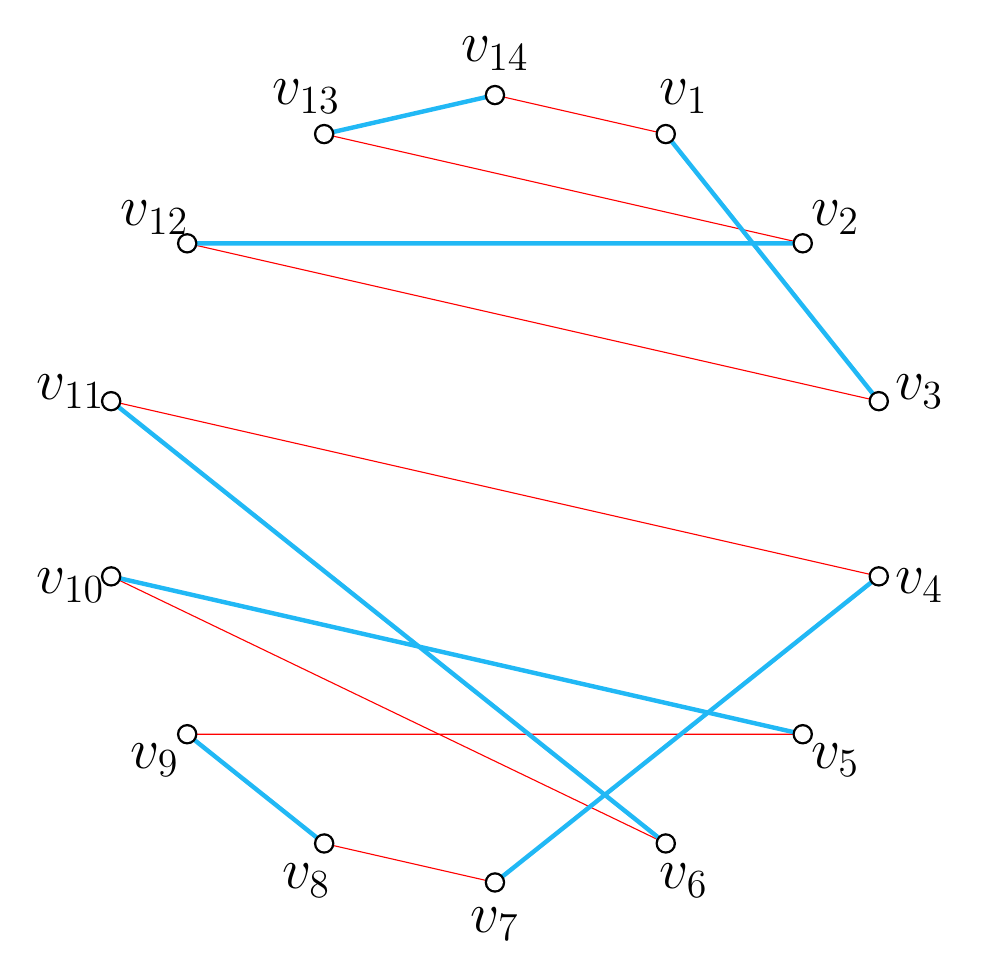
\begin{tikzpicture}
%Values of nodes:
% 0 = 1
% 1 = 1
% 2 = 2
% 3 = 2
% 4 = 3
% 5 = 3
% 6 = 4
% 7 = 4
% 8 = 4
% 9 = 5
% 10 = 6
% 11 = 7
% 12 = 7
% 13 = 7
% threshold tau = 7

%\foreach \n in {0,...,13}
\foreach \n in {1,...,14}
	\fill (90-\n*25.71428571:5cm) coordinate (v\n) circle [radius = 0.1]
		++(90-\n*25.71428571:15pt) node {\huge{$v_{\n}$}};
%\foreach \m/\n in {0/13, 1/12, 2/11, 3/10, 4/8, 5/9, 6/7}
\foreach \m/\n in {1/14, 2/13, 3/12, 4/11, 5/9, 6/10, 7/8}
	\draw [myRed] (v\n) -- (v\m);
%\foreach \m/\n in {0/2, 1/11, 3/6, 4/9, 5/10, 7/8, 12/13}
\foreach \m/\n in {1/3, 2/12, 4/7, 5/10, 6/11, 8/9, 13/14}
	\draw [ultra thick, myBlue] (v\n) -- (v\m);
%\foreach \n in {0,...,13}
\foreach \n in {1,...,14}
	\fill (90-\n*25.71428571:5cm) coordinate (v\n) circle [radius = 0.13];
%\foreach \n in {0,...,13}
\foreach \n in {1,...,14}
	\fill [white] (90-\n*25.71428571:5cm) coordinate (v\n) circle [radius = 0.1];

\end{tikzpicture}
	
\end{document}